\documentclass[11 pt]{report}

% Typography packages
\usepackage{microtype}
\usepackage[T1]{fontenc}
\usepackage{inconsolata}
\usepackage{fourier}
\usepackage{setspace}
\usepackage{textcomp}
\usepackage{booktabs}

% Math packages
\usepackage{amssymb}
\usepackage{amsmath}
\usepackage{bm} % Bold Greek math

% Figure and captioning packages
\usepackage[export]{adjustbox}
\usepackage[margin=0.1\textwidth]{caption} % Adjust caption text column margins
\usepackage{subcaption} % Subfigures with subcaptions
\usepackage{wrapfig} % Text wrapping around figures
\usepackage[export]{adjustbox} % Fine-tuned figure placement
\usepackage{float} % Control positioning of figures

% Algorithm packages
\usepackage{algorithm} % Algorithm environment
\usepackage{algorithmicx} % Improvements to Algorithm environment
\usepackage[noend]{algpseudocode} % No "end" statement at the end of an algorithm

% Other miscellaneous packages
\usepackage{array} % For fixed-length tables
\usepackage{graphicx}
\usepackage{hyperref}
\usepackage{todonotes} % DELETE WHEN FINISHED
\usepackage{verbatim} % DELETE WHEN FINISHED

\linespread{1.15}

\hypersetup{
    pdffitwindow=false,     % window fit to page when opened
    pdfstartview={FitH},    % fits the width of the page to the window
    pdftitle={Joshua Eddy MS Thesis},    % title
    pdfauthor={Joshua Eddy},     % author
    pdfnewwindow=true,      % links in new PDF window
    colorlinks=true,       % false: boxed links; true: colored links
    linkcolor=black,          % color of internal links (change box color with linkbordercolor)
    citecolor=black,        % color of links to bibliography
    filecolor=magenta,      % color of file links
    urlcolor=blue           % color of external links
}

% Control vertical spacing within matrices
\makeatletter
\renewcommand*\env@matrix[1][\arraystretch]{%
  \edef\arraystretch{#1}%
  \hskip -\arraycolsep
  \let\@ifnextchar\new@ifnextchar
  \array{*\c@MaxMatrixCols c}}
\makeatother

% Control the margins on block quotes
\newenvironment{myquote}[1]%
  {\list{}{\leftmargin=#1\rightmargin=#1}\item[]}%
  {\endlist}
  
\renewcommand{\arraystretch}{1.2}

\begin{document}

\thispagestyle{empty}

\begin{center}
{\Large 
A Hardware-Minimal Unscented Kalman Filter Framework for Visual-Inertial Navigation of Small Unmanned Aircraft
}
\vfill

Joshua Galen Eddy

\vfill

Thesis submitted to the Faculty of the \\
Virginia Polytechnic Institute and State University \\
in partial fulfillment of the requirements for the degree of

\vfill

Master of Science \\
in \\
Aerospace Engineering

\vfill

Kevin Kochersberger, Chair \\
Mazen Farhood \\
Craig Woolsey

\vfill

May 5, 2017 \\
Blacksburg, Virginia

\vfill

Keywords: Unscented Kalman Filter, SLAM, State Estimation, Localization,\\
Visual-Inertial Navigation, Unmanned Aircraft
\\
Copyright 2017, Joshua Galen Eddy
\end{center}

\pagebreak
\pagenumbering{roman}
\begin{center}
{\large 
A Hardware-Minimal Unscented Kalman Filter Framework for Visual-Inertial Navigation of Small Unmanned Aircraft
}

\vspace{2em}

Joshua Galen Eddy

\vspace{2em}

ABSTRACT

\vspace{1em}

\end{center}

This thesis presents the formulation and implementation of an Unscented Kalman Filter (UKF) framework for fusion of visual and inertial sensor data in unmanned aircraft navigation. Specifically, we fuse sensor readings from a 3-axis accelerometer, 3-axis gyroscope, and a Simultaneous Localization and Mapping (SLAM) algorithm to estimate the pose of an aircraft, such as a quadcopter, capable of hovering flight. We discuss the formulation of our UKF fusion algorithm, the development of a Robot Operating System (ROS) software package implementing the algorithm, and experiments in which this algorithm was used to track the motion of a physical vehicle simulating hovering flight in an indoor environment. In laboratory testing, the system was able to localize the test vehicle consistently with a mean total positional error of less than 7~cm and an overall maximum total error of less than 26~cm, as compared to the output of a Vicon motion capture system. We discuss possible applications of this system and future work that may build upon the results developed herein.

\thispagestyle{empty}

\pagebreak

\begin{center}
{\large 
A Hardware-Minimal Unscented Kalman Filter Framework for Visual-Inertial Navigation of Small Unmanned Aircraft
}

\vspace{2em}

Joshua Galen Eddy

\vspace{2em}

ABSTRACT (GENERAL AUDIENCE)

\vspace{1em}

\end{center}

This thesis presents the development and implementation of a software framework for estimating the position of a drone during flight. This framework is based on an algorithm known as the Unscented Kalman Filter (UKF), a recursive method of estimating the state of a highly nonlinear system, such as an aircraft. In this thesis, we present a UKF formulation specially designed for a quadcopter carrying an Inertial Measurement Unit (IMU) and a downward-facing camera. The UKF fuses data from each of these sensors to track the position of the quadcopter over time. This work supports a number of similar efforts in the robotics and aerospace communities to navigate in GPS-denied environments with minimal hardware and minimal computational complexity. The software framework explored in this thesis provides a means for roboticists to easily implement similar UKF-based state estimators for a wide variety of systems, including surface vessels, undersea vehicles, and automobiles. We test the system's effectiveness by comparing its position estimates to those of a commercial motion capture system and then discuss possible applications.

\thispagestyle{empty}

\input{Acknowledgments.tex}
\tableofcontents
\listoftables
\listoffigures
\chapter*{Acronyms}

\begin{description}
\item [AR] Augmented Reality
\item [EKF] Extended Kalman Filter
\item [GPS] Global Positioning System
\item [KF] Kalman Filter
\item [IMU] Inertial Measurement Unit
\item [MSF-EKF] Multi-Sensor Fusion Extended Kalman Filter
\item [PTAM] Parallel Tracking and Mapping
\item [SLAM] Simultaneous Localization and Mapping
\item [ROS] Robot Operating System
\item [UAS] Unmanned Aircraft System
\item [UAV] Unmanned Aerial Vehicle
\item [UKF] Unscented Kalman Filter
\item [UT] Unscented Transform
\item [UTM] Unmanned Traffic Management
\item [VIN] Visual-Inertial Navigation
\item [VO] Visual Odometry
\end{description}
\pagebreak

\pagenumbering{arabic}
\chapter{Introduction}

Until recently, the sensing and localization capabilities of small unmanned aerial vehicles (UAVs) have been computationally constrained due to restrictions on both the size and weight of sensors and onboard computer systems. Recent advances in miniaturized desktop computers, as well as low-power Graphics Processing Units (GPUs), have enabled a new class of computationally intensive algorithms to run onboard small aircraft without degrading flight time or other performance metrics. Specifically, small drones now present a viable platform for high-fidelity Simultaneous Localization and Mapping (SLAM), visual object recognition, and state estimation algorithms employing numerous heterogeneous sensors. In addition, the rising popularity of drones among hobbyists and researchers has fueled tremendous growth in the markets for brushless motors, electronic speed controllers, and airframes. With high-quality flight hardware and lightweight computers readily available, the arsenal of the robotics researcher has never been better stocked. The work detailed in this thesis is, in many ways, the product of these advantageous market conditions. With small aircraft capable of lifting heavier payloads and computers now lighter and smaller in footprint, demand is high for outfitting high-performance vehicles with top-notch sensing capabilities.

This work centers on an algorithm known as the Unscented Kalman Filter (UKF), a sensor fusion method for estimating the state of systems such as small aircraft. For years, this algorithm was inaccessible to roboticists and aerospace researchers alike due to its computational complexity. Computers capable of running the algorithm were simply too large, too heavy, and too power-hungry to be viable onboard components of small UAVs. The advent of smaller computers has changed this state of affairs. In this thesis, we present a formulation of the Unscented Kalman Filter aimed at estimating the pose of a quadcopter. This UKF formulation fuses outputs from only two sensors: an inertial measurement unit (IMU) and a downward-facing monocular camera. These two data streams are fused to estimate the vehicle's pose in real time. We propose this UKF framework as a hardware-minimal starting point for advanced multi-sensor fusion in UAV navigation.

\section{System Applications}

Applications for this system are wide-ranging, spanning virtually every conceivable use for a small drone. The following is a non-exhaustive list of possible applications:
\begin{enumerate}
    \item Mapping and 3D reconstruction of structures and topography,
    \item Emergency response,
    \item Infrastructure inspection,
    \item Autonomous package delivery, and
    \item Military/defense solutions.
\end{enumerate}
What all of these applications have in common is the need for robust localization. In each of the above scenarios, losing GPS could cause a crash. In such an event, the vehicle itself would pose a real threat to bystanders and property. Moreover, in the case of military aircraft, the vehicle could be captured by hostile forces.

\subsubsection{Mapping and 3D Reconstruction}

Growing demand for so-called ``precision agriculture'' has brought with it the need to map large areas of cropland at a high speed, with a low cost point. In the past, this need has been met by using satellite imagery and human-captured photography. With the arrival of low-cost drones, this work has been offloaded to aerial robots. Outfitted with specialized sensors such as hyperspectral cameras\footnote{\url{https://en.wikipedia.org/wiki/Hyperspectral_imaging}}, small UAS are now able to provide minute-by-minute coverage of large expanses of land. Moreover, these robots can be outfitted with reservoirs of pesticide or fertilizer and deployed to spray individual plants autonomously. It is in such roles that high-accuracy robust localization becomes a necessity. The accuracy required for precision agriculture can be obtained by utilizing the sensor fusion techniques discussed in this thesis.

The surfaces of buildings and other structures can be mapped in a similar fashion, given the appropriate sensors and the right framework by which to fuse them. 3D reconstruction has become popular among real estate agents, safety inspectors, and other parties with a vested interest in precise 3D renderings of large geometries. In this case, the aircraft must be able to localize itself precisely in order to take full advantage of onboard sense-and-avoid technologies. The ability of the aircraft to estimate its position is crucial to its ability to map hard-to-reach areas and maintain stable flight. Sensor fusion systems shine when GPS and other sensors are inevitably compromised by various environmental factors.

\subsubsection{Emergency Response}

UAS technologies have become a desirable tool for first responders in many parts of the world. The ability to deploy a UAV to survey forest fires or search for missing persons has been a game changer for law enforcement and emergency response teams. In the case of looking for survivors of a natural disaster, the requirements for an effective vehicle system are accurate localization and overall robustness. Vehicles sent into disaster areas will have to be able to navigate in sensor-compromising environments, sometimes at substantial speed. This use case highlights the need for redundant sensors and intelligent, failure-resistant sensor fusion.

\subsubsection{Infrastructure Inspection}

Infrastructure inspection is similar in many respects to 3D mapping. In both cases, small drones are preferable to manned aircraft because of their low cost, high maneuverability, and ease of use. Governments and private corporations alike have taken an interest in using small aircraft to automate the inspection of many types of infrastructure, including the following:
\begin{enumerate}
    \item Power lines,
    \item Oil rigs,
    \item Gas pipelines,
    \item Railroads, and
    \item Buildings.
\end{enumerate}
UAVs are an obvious ally to companies servicing most types of static infrastructure. Inspecting miles of wires or railroad track is a task well-suited to today's UAVs, which commonly ship with intuitive flight planning software. Operators---even those who have no experience flying remote-control aircraft---are now able to program missions and deploy drones with ease. The aircraft are able to survey miles of infrastructure regardless of conditions on the ground, such as flooding, ill-maintained roads, or wild animals. Operators with First-Person View (FPV) hardware can watch video streaming live from the aircraft as if they were onboard themselves. The need for robust localization here is obvious: the UAV cannot inspect anything to which it cannot navigate. Operating in the wilderness may require flying below the forest canopy or under natural overhangs that could block GPS reception. The same is true in urban environments, where tall buildings create so-called ``urban canyons'' which compromise GPS effectiveness. Large metal structures can also distort magnetometry readings and thus undermine the aircraft's ability to maintain its heading. In any case, UAVs used for large-scale inspections will be dependent upon intelligently combined sensing modalities.

\subsubsection{Autonomous Package Delivery}

A number of organizations, most notably Amazon\footnote{\url{https://www.amazon.com/Amazon-Prime-Air/b?node=8037720011}}, have made big bets on drones as the future of delivery services. The task of delivering goods to individual homes is no trifling matter. American homes come in all shapes and sizes and are surrounded by numerous structures and natural obstacles that could endanger a delivery aircraft and, by extension, the people and property nearby. Moreover, any drone delivery service would have to be predicated upon the ability of the UAV to land with sub-meter accuracy. Delivery drones will have to land precisely in cluttered environments amid dynamic obstacles. Visual sensing will be extremely important for identifying safe landing zones, avoiding power lines and fences, and surmounting other environmental challenges. GPS alone will not be enough to guide the vehicle safely in every conceivable circumstance. 

\subsubsection{Military/Defense Solutions}

Perhaps the most obvious application of a UKF fusion framework is in military operations, where precision navigation and robustness to sensor degradation are paramount for protecting soldiers in the field. As of the time of this writing, UAVs have been used in combat for years. However, augmented navigation could still make revolutionary contributions in areas such as
\begin{enumerate}
    \item Robust tracking of friendly and hostile elements,
    \item Remote observation of roads and vehicle-related hazards,
    \item Autonomous deliveries of materiel in-theater, and
    \item Human-machine teaming.
\end{enumerate}
Every combat zone will constitute a hostile environment for UAV operations, especially in the presence of GPS spoofing/jamming technologies. Combat UAVs will have to be able to tolerate multiple simultaneous sensor failures. Moreover, in-theater urban flight operations bring with them all of the same difficulties mentioned above, but with the added challenge of violent enemy interdiction. Robust sensor fusion could automate the task of operational overwatch and provide mission-critical intelligence in a timely manner---but only if the vehicle can localize itself reliably in sensor-hostile environments.

\section{Personal Motivation}

\textit{This section is largely comprised of background information regarding certain experiences leading up to, and motivating, the research developed in my thesis. This section does not contain any technical material, and is included only to provide context to the larger work.}

\vspace{1em}

\begin{wrapfigure}{r}{0.4\textwidth}
  \centering
    \includegraphics[width=0.4\textwidth]{CARD_gearREALLYBIG}
  \caption[CARD Team Logo]{The CARD team logo.}
  \label{fig:card_logo}
\end{wrapfigure}

I first took an interest in unmanned aircraft in the fall of 2012, my sophomore year of college. Several of my friends and I founded the Cooperative Autonomous Robotics Design (CARD) team at Virginia Tech in order to pursue our shared interest in autonomous vehicles. Our core team consisted of a dozen students devoted to designing and competing with drones and other robotic vehicles. Our team, guided by my future graduate adviser, Dr.~Kevin Kochersberger, entered two design competitions and brought home two awards for the university. We were also one of four university robotics teams selected by the Smithsonian Institution to participate in the opening ceremony for Robotics Week~2015. These early experiences with the team brought me into contact with new skills such as microcontroller programming, Proportional-Integral-Derivative (PID) controller design, basic mechatronics, and computer-aided design (CAD) modeling.

After two years of involvement with the CARD team, I applied for an internship at the National Institute of Aerospace\footnote{\url{http://www.nianet.org}} (NIA) in Hampton, Virginia. In the summer of 2014, I was part of a team of NIA researchers working on the Flying Donkey Challenge\footnote{\url{http://www.flyingdonkey.org}}, an international engineering competition centered around the idea of ``flying donkeys,'' full-sized autonomous airplanes capable of quickly carrying cargo between small airports in rural Africa. This competition, unfortunately now defunct, was divided into a number of sub-challenges focusing on different technical objectives such as precision landing and collision avoidance. Our team's goal was to design an inexpensive navigation system that could reliably guide unmanned aircraft during a Global Positioning System (GPS) blackout. This project introduced me to many of the technologies and techniques that would later become my major research interests, particularly the Robot Operating System\footnote{\url{http://wiki.ros.org}} (ROS), Kalman Filtering, and sensor fusion.

Through my internship at the NIA, I met Dr.~Danette Allen, head of the NASA Langley Autonomy Incubator. During my 2014--15 academic year, Dr.~Allen sponsored the CARD team to design and build two autonomous multirotor delivery drones. These aircraft were capable of delivering 5\nobreakdash-lb packages to distances of up to 2.5~miles (or 5~miles, round trip). In addition, these vehicles were able to land precisely on 1~m$^2$ April tags, a type of visual marker used in augmented reality applications. Following the completion of this project, I worked as a summer intern at the Autonomy Incubator, thereby further advancing my interest in Kalman filtering, sensor fusion, and visual localization.

During the summer of 2015, I began the research that evolved into my thesis project, studying Visual-Inertial Navigation (VIN) and the Unscented Kalman Filter (UKF). As I read more and more on these subjects, I became interested in the design of the algorithm underlying the UKF. Unlike many other formulations of the Kalman Filter, the UKF has a notably limited dependence on information about the system under scrutiny (this \textit{system agnosticism} is discussed in more detail in Chapter~\ref{ch:Alg_Design}). The more I learned about the UKF, the more I became excited about the idea of taking advantage of this limited dependence trait to build a minimalistic software interface by which a wide variety of disparate systems could be tracked and studied in a ROS framework. I envisioned a ``one-stop shopping'' experience for massively reusable and customizable filtering profiles that could fulfill the needs of researchers and roboticists who may have little knowledge of state estimation techniques. This vision eventually drove my development of the \texttt{kalman\_sense} ROS package, cementing my interest in unmanned aerial vehicle (UAV) state estimation processes and controls.


\section{Organization of this Document}

\subsection*{Prior Work}

In Prior Work, we explore recent contributions to loosely coupled filter-based navigation and state estimation processes. We focus primarily on a number of impactful publications coming from the Autonomous Systems Lab\footnote{\url{www.asl.ethz.ch}} (ASL) at ETH~Zurich\footnote{\textit{Eidgen{\"o}ssische Technische Hochschule Z{\"u}rich}, the Swiss Federal Institute of Technology in Zurich.} and the University of Pennsylvania's GRASP Lab\footnote{\url{www.grasp.upenn.edu}}. We define the current state of the art in filter-based navigation and establish the research context in which this thesis exists.

\subsection*{Algorithm Design and Implementation}

Because of the algorithmic nature of state estimation processes, we explore in detail the design and implementation of the \texttt{kalman\_sense} ROS package. We discuss plant model abstraction as well as code organization and data flow and then summarize the process by which one could extend \texttt{kalman\_sense}'s functionality and the advantages of system-agnostic algorithm design.

\subsection*{Experimental Design}

In this section, we first establish the goals of the testing regimen and then discuss the real-world execution of these goals. We discuss important statistical methods for characterizing the system's effectiveness as well as data collection procedures and post-processing. The system's physical testing infrastructure is explored in detail.

\subsection*{Experimental Results}

In Experimental Results, we evaluate the system's performance during testing and seek out any limiting factors that influence estimation accuracy. We probe for possible improvements to the algorithm and provide a notional understanding of the system's theoretical effectiveness in real-world scenarios.

\subsection*{Conclusions and Future Work}

We summarize the contributions made in this thesis, the effectiveness of the \texttt{kalman\_sense} ROS package, and the insights acquired during programming and testing. We explore avenues for future research as well as possible improvements to the existing system.
\chapter{Prior Work}

\section{Development of the Unscented Kalman Filter}

In \cite{Julier1997}, Simon Julier and Jeffrey Uhlmann discuss the development and demonstration of a new nonlinear estimator for the Kalman Filter. Recognizing that most applications for autonomous navigation are fundamentally nonlinear in both their dynamics and their observation models, Julier and Uhlmann proposed the use of a set of discretely sampled ``sigma points'' to determine the mean and covariance of a probability distribution. By recasting the prediction and correction steps of the Kalman filter in the form of unscented transforms (UTs), this new filter eliminates the need to calculate Jacobian matrices. Julier and Uhlmann argued that for this reason their formulation was easier to implement than the Extended Kalman Filter (EKF) and went on to suggest that its use could supplant the EKF in virtually all applications, linear or nonlinear.

In \cite{Julier1998}, Julier acknowledges that the (linear) Kalman Filter has been used successfully in many nonlinear scenarios, but points out that the use of only the first two moments of the state estimate sigma points results in neglect of all higher order information (that is, third-order moments, or ``skew''), a potentially rich source of new and useful information relating to symmetry of the state estimate. By extending the sigma point selection scheme of the conventional unscented transform, Julier was able to present a tractable but computationally complex extension of the Kalman filter that could predict not only the first two moments of a sigma point distribution, but also the skew. Though formulated initially for unimodal distributions, Julier stated that the approach could, with additional mathematical considerations, be generalized for use with multimodal distributions. Julier's contention was that use of higher order information could promote better performance levels in autonomous vehicle navigation. The utility of maintaining and utilizing higher order information through the use of skewed filtering was assessed by the authors in a realistic tracking scenario. However, the results turned out to be somewhat disappointing as the change in performance turned out to be minimal, presumably due to the linearity of the filter's update rule. Accordingly, research in this area continues, including examination of the use of nonlinear update rules in the filtering process.

In \cite{Julier2002}, Julier describes a novel approach to modifying the unscented transformation state estimation method, a subject of one of his previous studies in collaboration with Uhlmann. In the current paper, however, Julier takes the additional step of introducing a new framework for scaling sigma points as part of the state estimation process. The general framework of the new methodology allows preservation of the first two moments of any set of sigma points, thus providing a construct for limiting values to either the conventional unscented transform or the modified (scaled) transform. Providing detailed mathematical validations, the author shows that the new scaling algorithm is computationally manageable in that it is, in essence, little more than the conventional unscented transformation algorithm with the addition of a simple post-processing step, the only difference being the inclusion of an extra correction term. Thus, the new algorithm's computational and storage costs are similar to that of the non-scaled transformation. The performance level of the scaled UT is thus demonstrably superior when the conventional non-scaled UT is used for propagating the two lower-order moments of a sigma point distribution.

In \cite{Julier2004} Julier and Uhlmann discuss the application of the extended Kalman filter (EKF) as an estimation algorithm and the associated difficulties. Because the EKF is fundamentally a linearizing approach to estimation, its effectiveness is thus tied to the veracity of the local linearity assumption for the system under scrutiny. These limitations led to the development of the unscented transformation (UT) for nonlinear applications. In this paper, Julier and Uhlmann describe the unscented transformation (UT) and its benefits, including easier implementation and improved accuracy. The UT offers greater accuracy and reliability by applying higher order information using sigma points to the traditional mean and covariance information associated with linear applications. The authors provide examples, which may be tailored, that show how the UT overcomes the limitations of the EKF.

\section{Kalman Filtering for Robotic Navigation and State Estimation}

[Mourikis 2007] Mourikis et al. expand investigation of the familiar topic of Vision-aided Inertial Navigation, with particular emphasis on small, low-cost, low-weight systems, including unmanned aerial vehicles (UAVs) using a monocular camera. Because technical advances have been made in the manufacture of inertial sensors, these robotic systems are capable of producing high precision state estimations even in uncontrolled urban environments, without utilizing a 3D feature position in the filter state vector of the Extended Kalman Filter. The exceptional accuracy produced in this real-time, real-world pose estimation model is highly desirable because it produces images that are rich in high-dimensional measurements. This robustness, however, invariably comes at a cost of computational complexity in the EKF-based algorithm, a trade-off that is unavoidable in the present state-of-the-art for vision-aided inertial navigation systems.

[Safanov 2007] Safonov revisits the decade of the 1970s, a period of transition in the theoretical framework underlying effective control of dynamic motion, marking a paradigm shift from a long-held theoretical construct centered on the ``optimality'' of Linear-Quadratic-Gaussian (LQG) feedback design theory to one centered on ``robustness.'' The author observes that the shift stems from the poor performance of the LQG controllers involving early tests in real-world scenarios, a problem later recognized as an inadequate level of attention to the real-world need for high-level performance with respect to accuracy, flexibility, and overall robustness in motion control. A more pragmatic approach to motion control theory was thus born, with significant milestones being achieved throughout the 1970s, including advancements in the areas of diagonally structured uncertainty, LQ multivariable gain margins, and LQ phase-margins, to name just a few. Further advancements came in the 1980s, culminating in the publication of the ``Robust Control Toolbox'' in 1988, thus making robust control design techniques widely available to students and engineers alike.

[Klein, 2007] In most Augmented Reality (AR) camera pose estimate scenarios, there exists at least some knowledge of the user environment. Complications arise when this is not the case. In this paper, Klein and Murray propose a method in which a user can track a calibrated hand-held camera in an unknown environment, while still building a map of the environment. Primarily useful only for small AR workspace areas, this design splits the tracking and mapping functions into two separate tasks. These two tasks are processed on a dual-core computer utilizing ``parallel threads,'' with one thread directly tracking erratic motion of the hand-held camera while the other thread simultaneously produces a 3D map of the environment. In this approach, the authors estimate a dominant plane from mapped points and then populate it with virtual characters. To simplify the computationally complex tasks of simultaneously tracking and mapping, the nature of the scene to be tracked and mapped was constrained:  it should be small and, for the most part, static. Experiments demonstrated that the system could produce highly accurate maps, rich in detailed landmark information trackable at frame rate, all without prior knowledge of the scene and with minimal initialization procedures.

In [Weiss2010], Weiss et al. discuss how autonomous micro aerial vehicles (MAVs) provide access to environments that are otherwise difficult to traverse. Further, they mitigate the risk to people and the environment. For many applications, the MAV must navigate in a GPS-denied environment. This paper presents an approach to navigation that relies on a micro helicopter, a single camera, and onboard inertial sensors. A monocular simultaneous localization and mapping (SLAM) framework stabilizes the vehicle, which is used to overcome the issues with drift. This research is important because urban canyons limit GPS availability. The authors, in this paper, show that autonomous navigation in a GPS-denied environment is achievable. 

[Shen 2011] Shen et al. extend the work of other authors on the topic of autonomous MAV navigation, particularly as it relates to stable indoor flight and GPS-denied localization in constrained multi-floor environments. The research distinguishes itself by emphasizing the use of onboard sensors only, as well as fully autonomous, real-time internal computational capabilities, with no hands-on user interaction beyond basic high-level commands. The research extends to multi-floor MAV operation with loop closure. It also addresses specially designed controllers to help compensate for sudden changes in wind velocity and air flow as the MAV traverses constrained low-clearance areas with potentially strong aerodynamic disturbances.

[Weiss2011] Weiss and Roland Siegwart developed an algorithm that provides a metric scale to estimate that estimates monocular visual odometry or monoSLAM approaches. The authors accomplished the development of the metric scale by the addition of an inertial sensor with a three-axis accelerometer and gyroscope. Stephan Weiss and Roland Siegwart created a modular solution that is based on an Extended Kalman Filter (EKF) and provides both simulated results and data-based results. In this paper, the authors discuss their unique approach, its applications, versatility, and reliability of their estimating algorithm for visual odometry, such as visual SLAM, in real-time. 

[Weiss 2012] Weiss et al. present a versatile framework to enable autonomous flights of a Micro Aerial Vehicle (MAV). The MAV has only slow, noisy, delayed and possibly arbitrarily scaled measurements available. The use of these measurements directly for position control is not practical since MAVs exhibit great agility in motion. In addition, these measurements often come from a selection of different onboard sensors, hence accurate calibration is crucial to the robustness of the estimation processes. In this article, Weiss, et al. address the problems using an EKF formulation which fuses these measurements with inertial sensors. The authors not only estimate pose and velocity of the MAV, but also estimate sensor biases, scale of the position measurement and self (inter-sensor) calibration in real-time. The authors show that it is possible to obtain a yaw estimate from position measurements only. The authors demonstrate that the proposed framework is capable of running entirely onboard a MAV performing state prediction at the rate of 1 kHz. Their results illustrate that this approach is able to handle measurement delays (up to 500 ms), noise (std. deviation up to 20 cm) and slow update rates (as low as 1 Hz) while dynamic maneuvers are still possible. Stephan Weiss et al. present a detailed quantitative performance evaluation of the real system under the influence of different disturbance parameters and different sensor setups to highlight the versatility of our approach. 

[Weiss, Achtelik 2012] Weiss et al. explore the advantages of utilizing a high-performance navigation algorithm on a low-cost, low-weight micro aerial vehicle (MAV) equipped with a single camera and an inertial measurement unit (IMU) capable of both onboard processing and real-time operations, with focus on a speed estimation module to help control the speed of the MAV, all within an Extended Kalman Filter framework. The system was shown to be useful for real-time self-calibration of the sensor suite – critical to ensuring the robustness and flexibility of any state estimation process – and as a potential solution to some of the tracking failures common to keyframe-based modules. 

[Huang 2013] Huang et al. explore solutions to two Unscented Kalman Filter (UKF) limitations that exist in current state-of-the-art Simultaneous Localization and Mapping (SLAM) systems. Specifically, the authors address the problems of cubic complexity in the number of state pose estimates, and the inconsistencies in those estimates caused by a mismatch between the observability properties of statistically-linearized UKF systems and the observability properties of nonlinear systems. To address the problem of cubic complexity, the authors introduce a novel sampling strategy which produces a constant computational cost which, while linear in the propagation phase, is quadratic in the update phase. Although this new sampling strategy was primarily proposed for resolving the above-referenced SLAM problem, it also has potential usefulness in other nonlinear estimation applications. To address the problem of inconsistency in state estimations, the authors propose a new UKF algorithm which, due to the imposition of observability constraints, ensures that the linear regression computations of the modified UKF system produce results similar to those of nonlinear SLAM systems and, in the process, provide improved accuracy and consistency in state estimations. Importantly, these results have been validated with both real-world and simulation experiments. While the paper focused on 2D SLAM, the authors contend that their proposed methodology is also useful for robot localization in 3D, using inertial sensors.

[Lynen 2013] Lynen et al. report on the development of a generic framework to overcome known limitations in fusing information transmitted from multiple sensors in the navigation of robots, focusing mainly on the navigational needs of rotor-based micro aerial vehicles (MAV) which can more easily traverse from indoor to outdoor domains. The authors demonstrate that their Multi-Sensor-Fusion Extended Kalman Filter framework is capable of processing various measurements from an unlimited number of sensors, as well as sensor types, while simultaneously performing online self-calibrations of the overall sensor suite. Designed to be modular, the framework allows seamless handling of sensor signals during operation while performing other complex, iterative calculations to achieve near optimal linearization points for state updates. 

[Engel 2013] Engel et al. propose a novel direct monocular Simultaneous Localization and Mapping (SLAM) algorithm unlike that of existing direct approaches which embrace pure visual odometry. The novelty of the authors' approach is that it permits the building of consistent, accurate, large-scale 3D maps of the environment while simultaneously tracking camera motion, incorporating any scale-drift in the environment and allowing for the detection and correction of any accumulated drift. The system is capable of running real-time on a central processing unit and as visual odometry on a modern smartphone.

[Rogers III 2014] Rogers et al. presented a methodology for overcoming some of the constraining conditions encountered in a GPS-guided autonomous robotic system, such as occlusion (blocking of GPS signals) and multipath (reception of indirect signals due to environmental reflections) and potentially to ameliorate the effects of jamming or spoofing resulting from adversarial activities. Specifically, the methodology incorporated GPS measurements into a feature-based mapping system, thus providing geo-referenced coordinates allowing for better execution of high-level missions and providing the ability to correct accumulated mapping errors over the course of long-term operations in both indoor and outdoor environments.

[Hesch 2014] Hesch et al. investigated the relationship between system observability properties and estimator inconsistency for a Vision-aided Inertial Navigation System (VINS). By factorizing the observability matrix according to the observable and unobservable modes, they produced a new methodology for determining the unobservable directions of nonlinear systems. They then applied this new method to the VINS nonlinear model to determine analytically any of its unobservable directions. Subsequently, they leveraged their analysis to improve both the accuracy and consistency of linearized estimators as they applied to VINS. Through the use of extensive simulations and validation testing, the key findings of the analysis were evaluated for the purpose of demonstrating the superior accuracy and consistency of the proposed VINS framework.

[Faessler 2015] Faessler et al. report on the development and demonstration of a low-cost, low-weight, vision-based quadrotor micro aerial vehicle (MAV) with onboard sensing, computation, and control capabilities. These onboard capabilities eliminated reliance on external positioning systems such as GPS or motion capture systems. This development moves the MAV from its current line-of-sight control state to wireless communications with the ability to execute intricate processes autonomously and to transmit live feedback to a user. Reporting on both indoor and outdoor experiments, the authors believe that such a vehicle potentially would be a great enhancement in search-and-rescue missions, disaster response, and remote inspection of terrain. 

\chapter{Algorithm Design and Implementation} \label{ch:alg_design}

\section{UKF Formulation}

We begin by defining the following vector quantities:
%
\begin{equation}
tk: p, q, v, \omega, a
\end{equation}
%
tk: define n and m


We then define the state vector $\mathbf{x} \in \mathbb{R}^{n}$:
%
\begin{equation}
\mathbf{x} \triangleq \left\lbrace
\mathbf{p},
\mathbf{q},
\mathbf{v},
\mathbf{\omega},
\mathbf{a},
\right\rbrace ^{T}.
\end{equation}
%
The covariance associated with each state $\mathbf{x}$ is a matrix $\mathbf{P} \in \mathbb{R}^{n \times n}$. A set of $2n + 1$ sigma points is then derived from $\mathbf{x}$ and $\mathbf{P}$:
%
\begin{align}
\mathbf{\chi}^{0} &= \mathbf{x} \nonumber\\
\mathbf{\chi}^{i} &= \mathbf{x} + \left( \sqrt{\left( n + \lambda \right) \mathbf{P} } \right)_{i}, \quad i = 1, \dots, n \\
\mathbf{\chi}^{i} &= \mathbf{x} - \left( \sqrt{\left( n + \lambda \right) \mathbf{P} } \right)_{i-n}, \quad i = n+1, \dots, 2n \nonumber
\end{align}
%
where $\lambda$ is defined in terms of the following constants:
%
\begin{equation}
tk: \alpha, \beta, \kappa, \lambda
\end{equation}

tk: TO BE CONT'D.

\section{Software Design Considerations}

Much of the impetus for creating the \texttt{kalman\_sense} package came from a desire to create a generic UKF framework for estimating the state of arbitrary systems using any number of relative and absolute sensors. To achieve this, the \texttt{kalman\_sense} package is organized in an object-oriented manner around an overarching abstract class called \texttt{UnscentedKf}. This abstract class contains a number of methods performing the different mathematical operations defined in Section~\ref{sec:ukf_formulation}. These methods have been written in a generic manner in order to enable easy extension of \texttt{UnscentedKf} by other subclasses containing concrete implementations of various systems. Currently, the package contains exactly one such subclass, known as \texttt{QuadUkf}. This subclass contains methods and data structures related directly to estimating the state of a quadcopter or other rotorcraft UAV.

This object-oriented architecture is meant to allow for a certain degree of system agnosticism. The abstract \texttt{UnscentedKf} class encapsulates the generic mathematics of the Unscented Kalman Filter without knowledge of particular system constraints. This class does little other than matrix mathematics and is designed to take as input the number of a system's states $n$ and its number of sensors $m$. With this knowledge, \texttt{UnscentedKf} is able to populate a set of mean and covariance weights and intelligently perform all of the requisite linear algebra for the UKF formulation. All other knowledge of particular states, sensors, vehicle geometry, and other particulars is hidden within subclasses such as \texttt{QuadUkf}.

\texttt{UnscentedKf} behaves in a manner similar to a Java interface in that it requires the extending class to supply functions codifying a process model and an observation model for the system under scrutiny. These two functions, along with $n$ and $m$, form the entirety of what \texttt{UnscentedKf} ``knows about the vehicle.'' All other details, including the fact that the class is being used in a ROS environment, are hidden from \texttt{UnscentedKf}. It is worth noting that \texttt{UnscentedKf}'s only dependency is on the Eigen\footnote{\url{www.eigen.tuxfamily.org}} C++ linear algebra library.

The subclass (\texttt{QuadUkf} for the remainder of this thesis) handles all of the ROS communications for the given system. Specifically, this class has callback functions for receiving sensor data and is responsible for publishing state and covariance estimates. The \texttt{kalman\_sense} \texttt{main} method handles setup and teardown of the necessary ROS publisher and subscriber nodes.


\chapter{Experimental Design} \label{ch:Exp_Design}

\section{Testing Considerations}

Before venturing further, we should summarize the goals of the UKF framework described previously, paying particular attention to unmanned aircraft system (UAS) operations. This ROS package was designed with the express intent of producing estimates of the position vector $\mathbf{p}$ and orientation quaternion $\mathbf{q}$ of a rotorcraft UAV in real time. Thus, the experiments testing the system's efficacy compare the filter's estimates of position and orientation to the ground truth measured by Vicon.

\begin{figure}[t]
    \centering
    \begin{subfigure}[t]{0.5\textwidth}
        \centering
        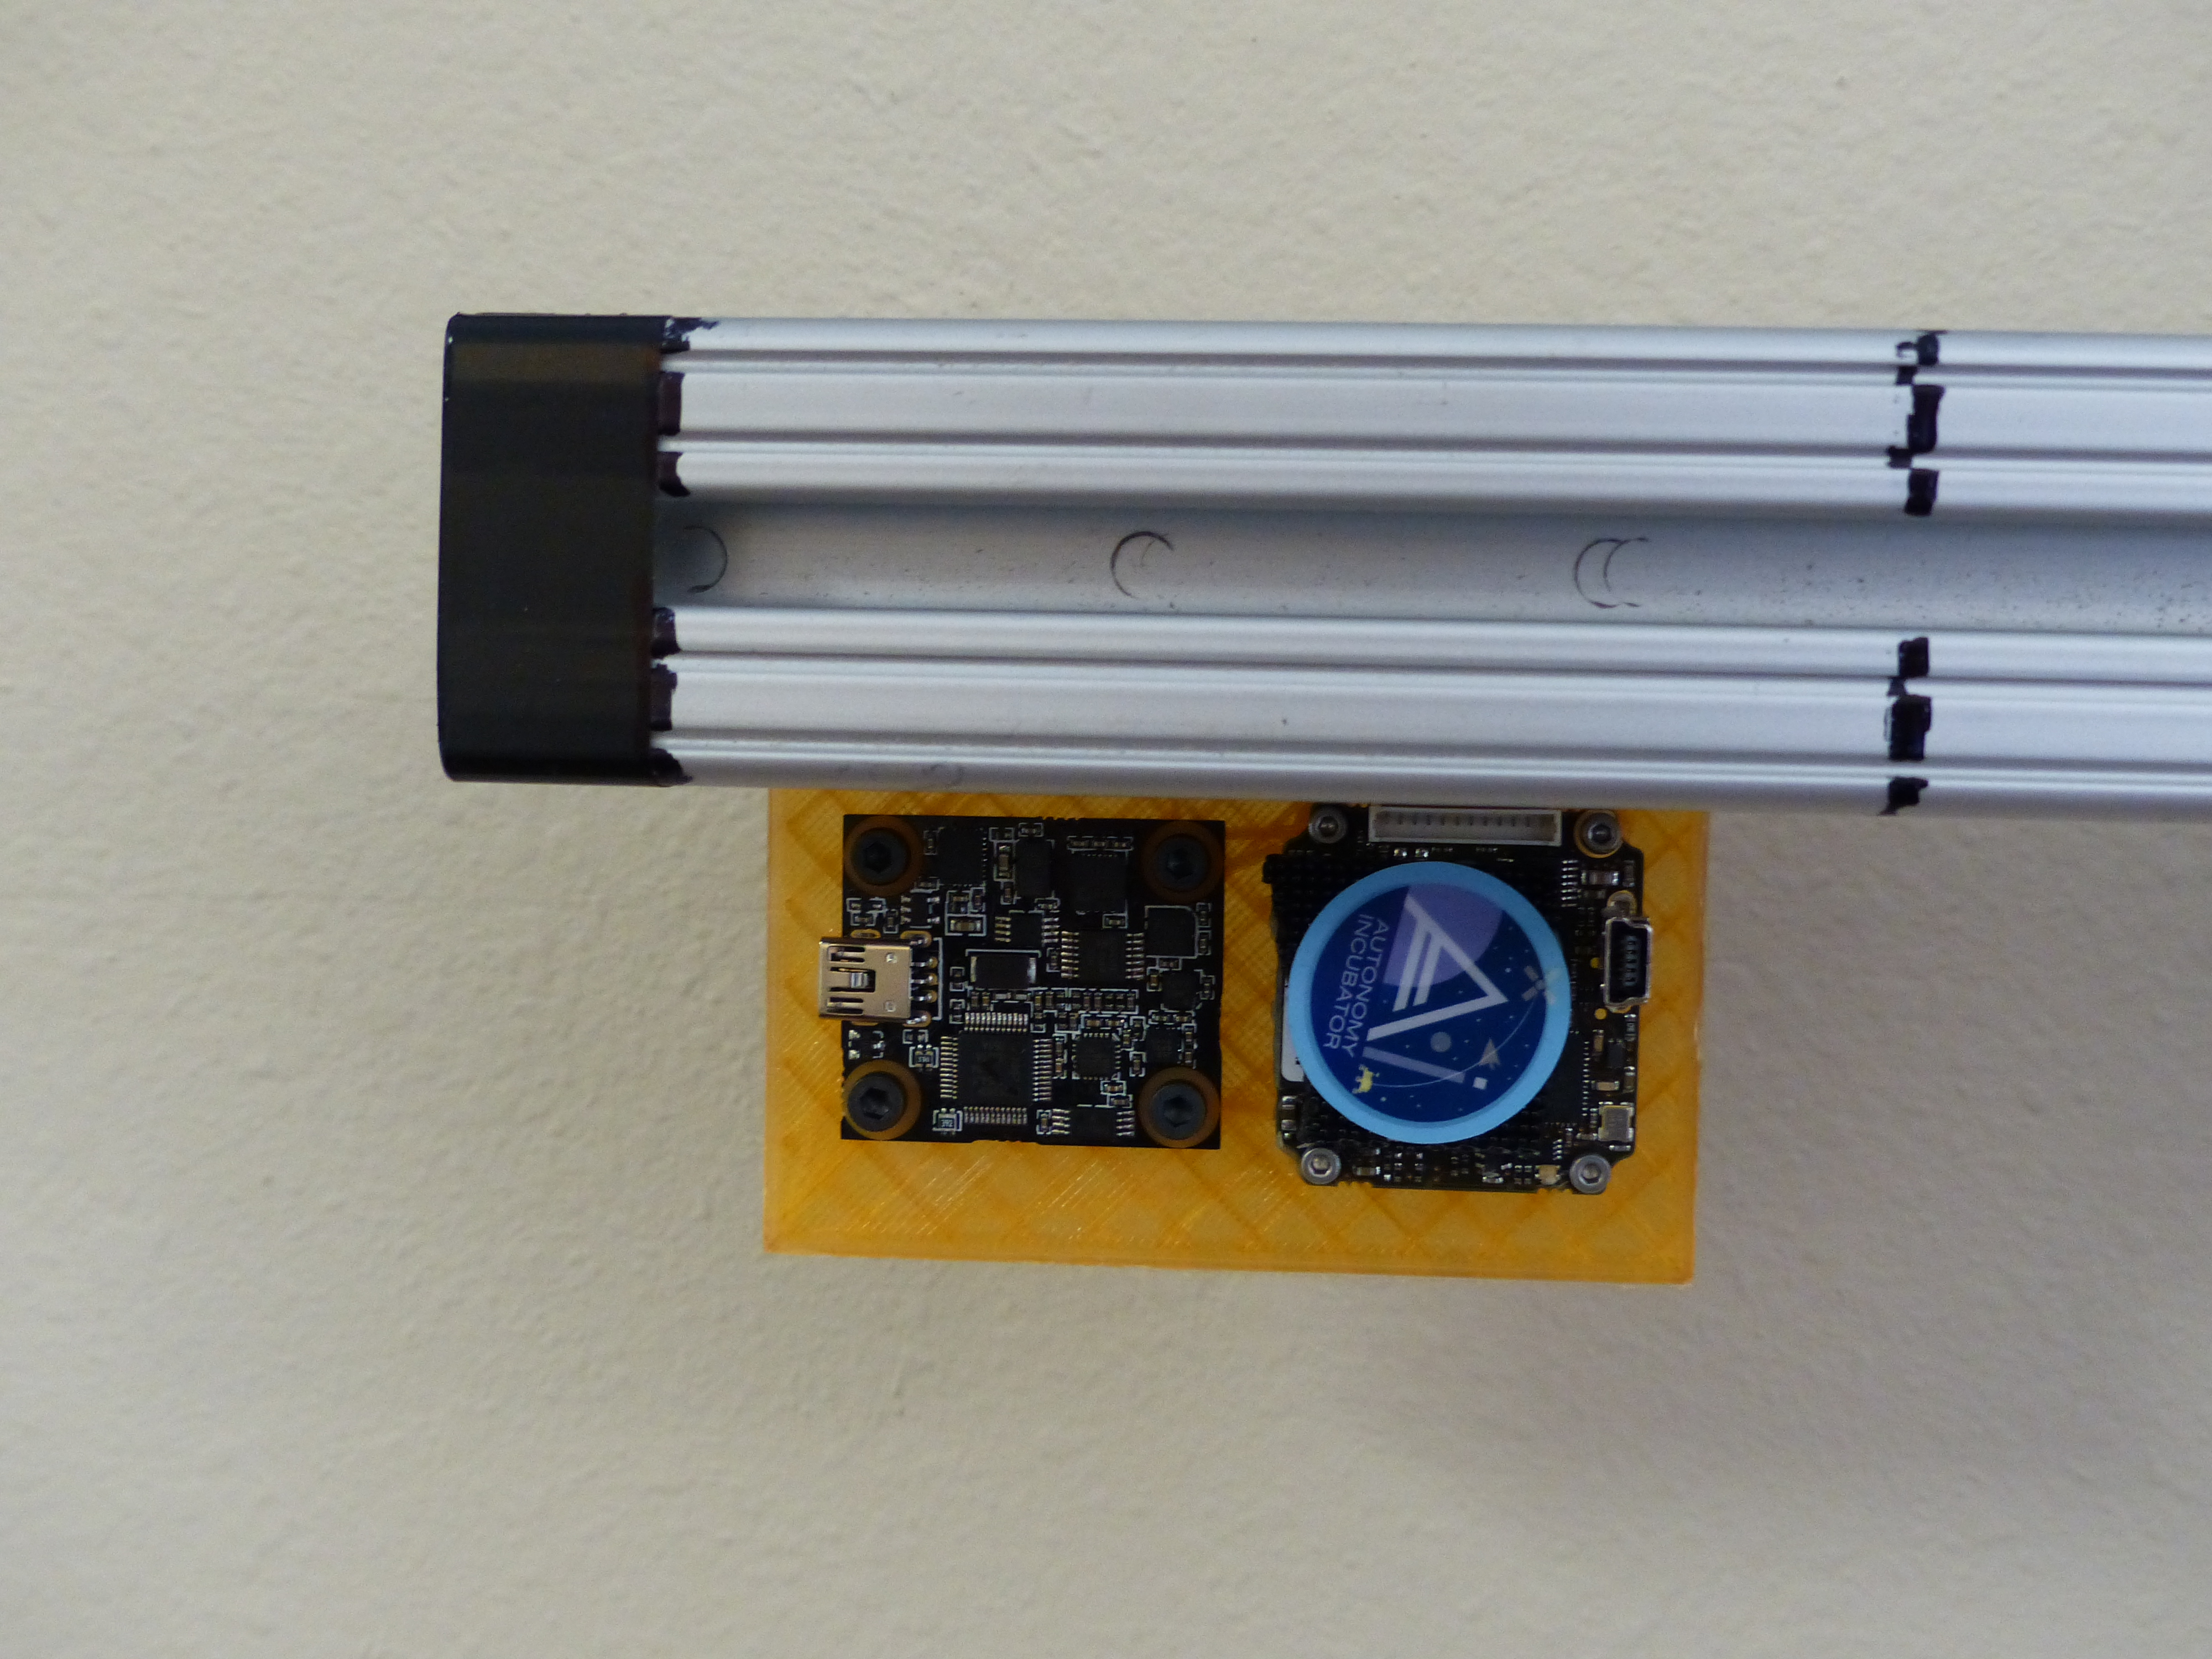
\includegraphics[width=0.8\textwidth]{sensor_mount_top}
        \caption{Top view of sensor mount.}
    \end{subfigure}%
    ~ 
    \begin{subfigure}[t]{0.5\textwidth}
        \centering
        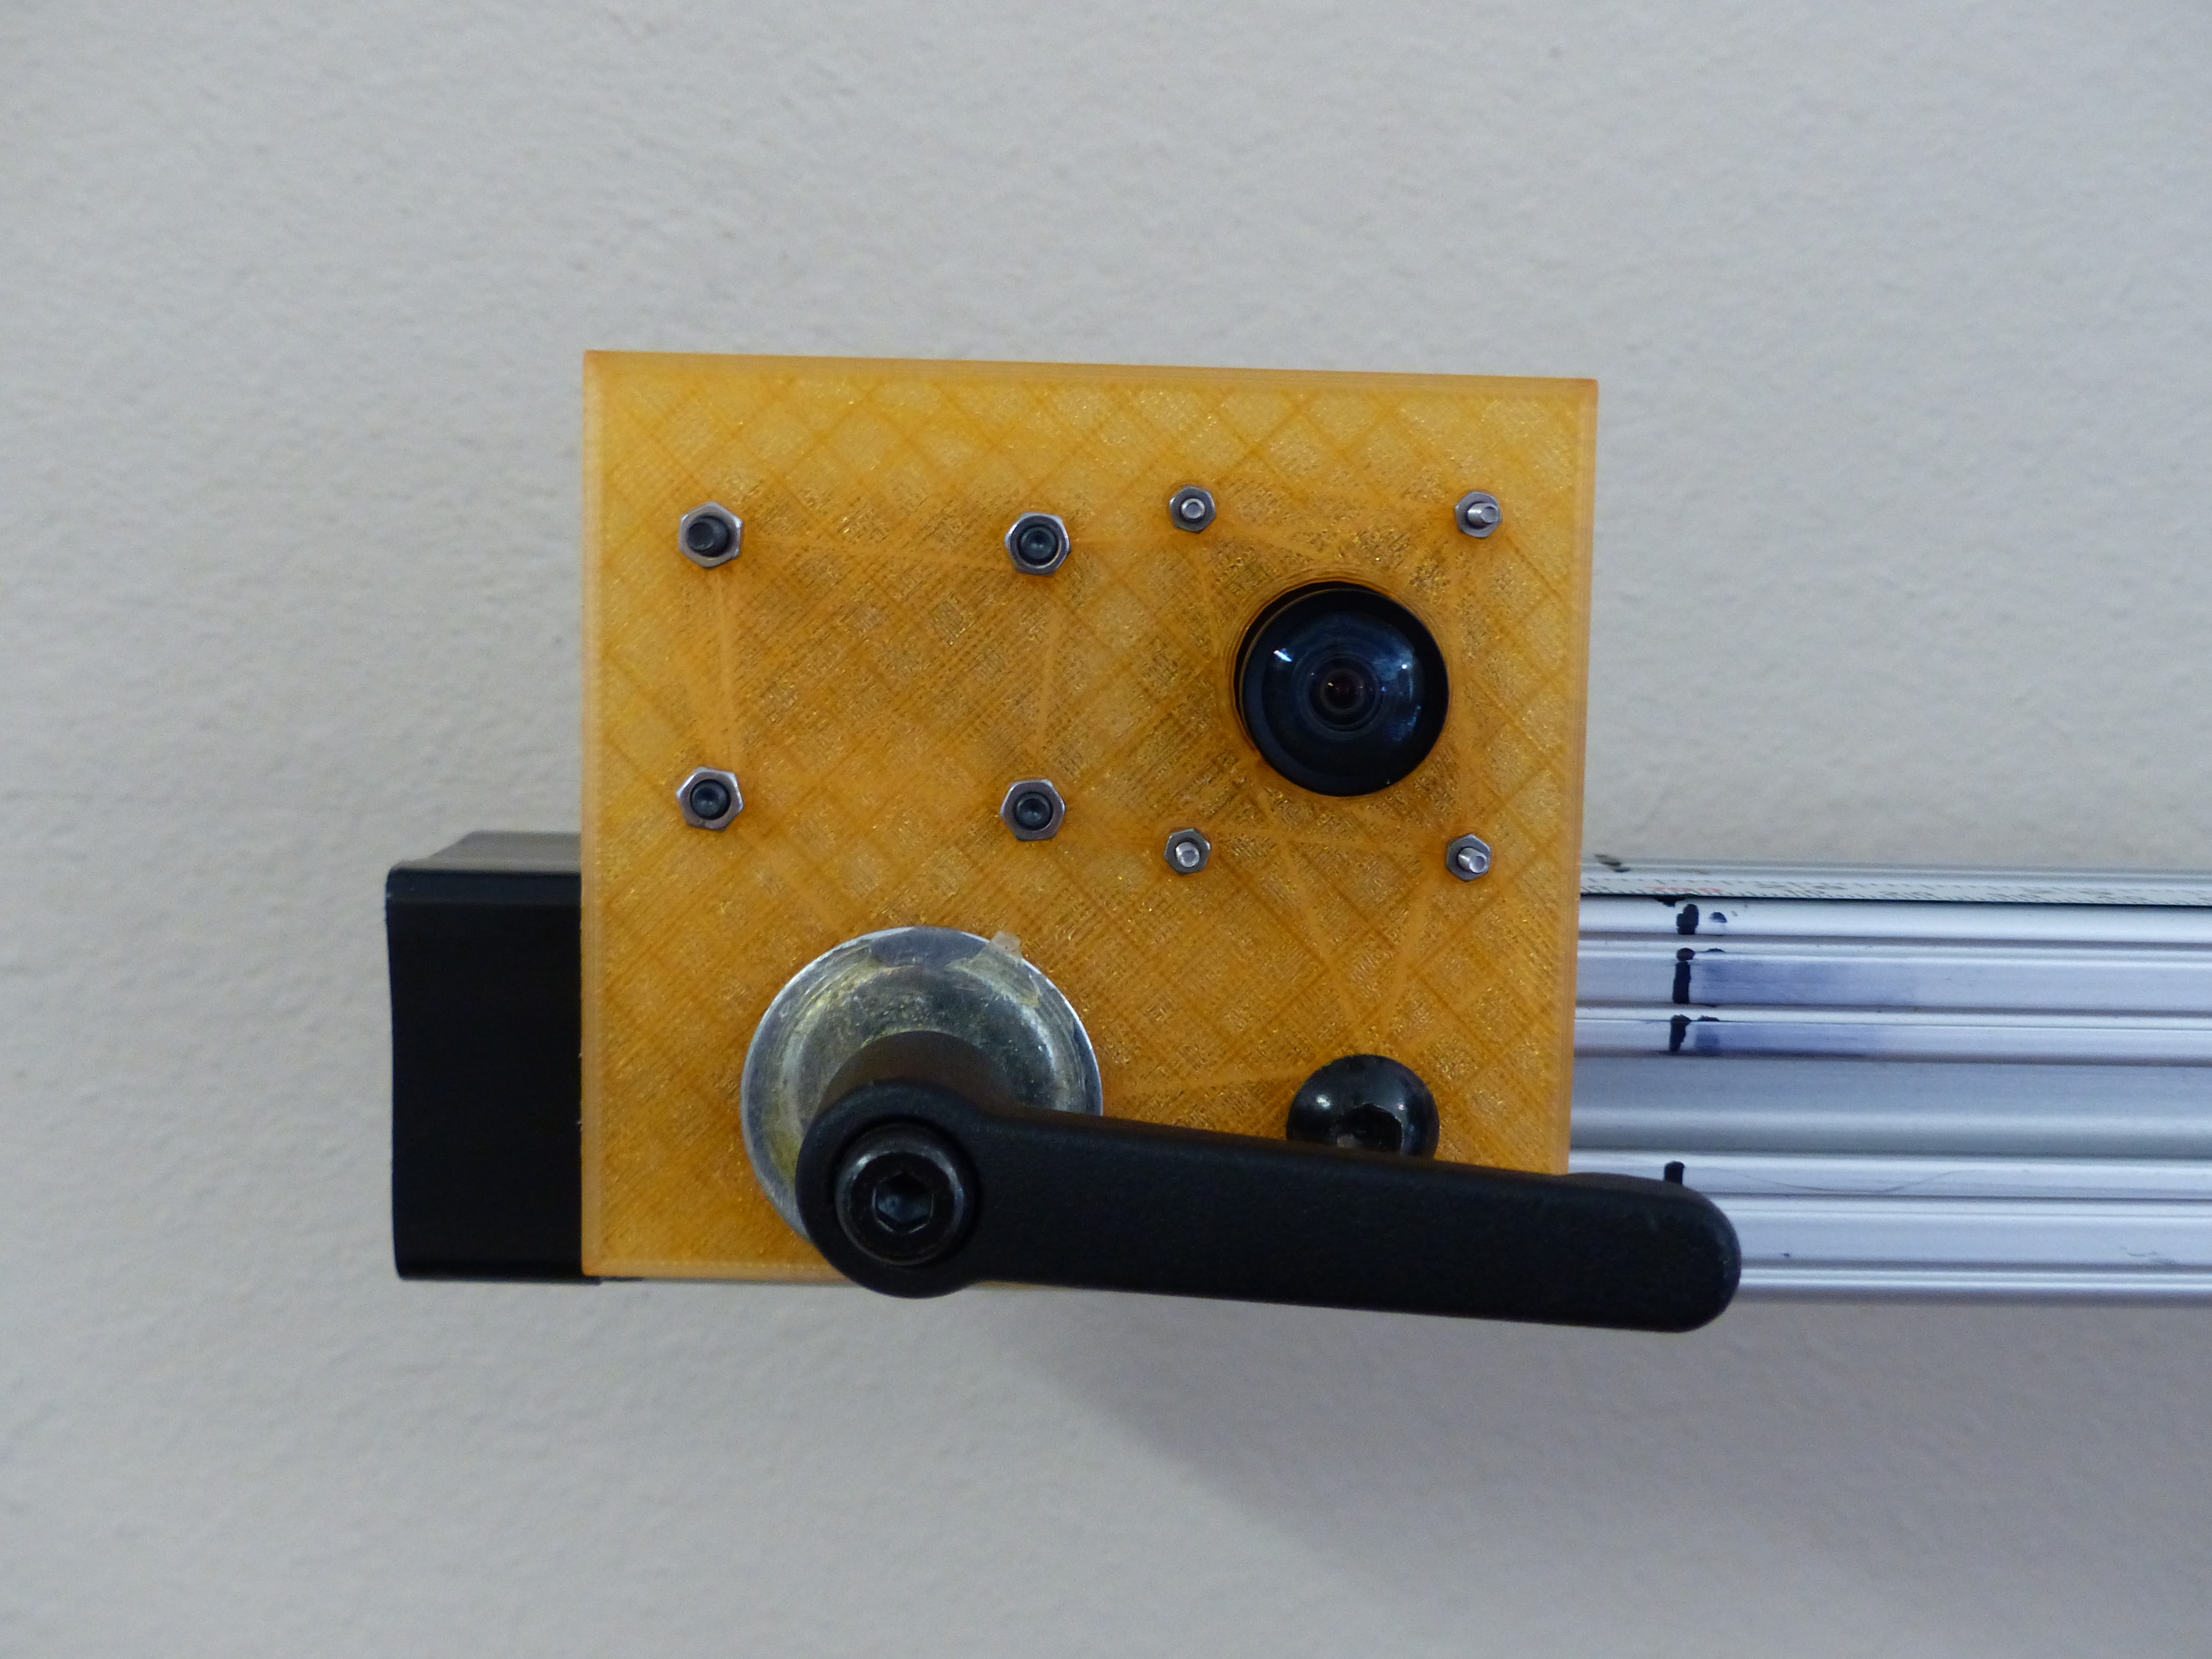
\includegraphics[width=0.8\textwidth]{sensor_mount_bottom}
        \caption{Bottom view of sensor mount.}
    \end{subfigure}
    \caption[3D-printed sensor mount]{The 3D-printed sensor mount. In (a), the Phidgets IMU is on the left and the mvBlueFOX camera is on the right. In (b), the linear braking handle is visible.}
    \label{fig:sensor_mount}
\end{figure}

This system depends upon two sensors: a single global-shutter camera and an IMU. The IMU used in this experiment contains a 3-axis accelerometer and 3-axis gyroscope. To simulate both sensors moving through the scene in a manner reminiscent of hovering rotorcraft flight, a rolling test stand was constructed to carry the sensors safely throughout a large motion capture environment. Mounting the sensor suite on a large, steady, level platform allows for a high degree of control over the accelerations and angular velocities felt by the IMU, as well as the motion captured by the ventral camera. In order to validate the UKF framework's effectiveness under ideal conditions, a modern laptop computer containing an Intel i7 processor with 16~GB of RAM was used for all computations. The floor of the motion capture environment was strewn with a mixture of April tags and modified Quick Response\footnote{\url{https://en.wikipedia.org/wiki/QR_code}} (QR) codes in order to provide sufficient visual features for PTAM to track.

\section{Materials}
\subsection{Computation and Sensing}
\begin{enumerate}
\item One (1) MatrixVision mvBlueFOX-MLC Camera\footnote{\url{https://www.matrix-vision.com/USB2.0-single-board-camera-mvbluefox-mlc.html}}
\item One (1) 1044\_0 PhidgetSpatial Precision 3/3/3 High Resolution IMU\footnote{\url{http://www.phidgets.com/products.php?product_id=1044}}
\item One (1) Hewlett-Packard Spectre x360 Convertible Laptop 13-ac076nr\footnote{\url{http://store.hp.com/us/en/pdp/hp-spectre-x360---13-ac076nr}}
\item Two (2) male Mini USB 2.0 to male USB Type A cables
\end{enumerate}

\subsection{Mobile Test Stand}
\begin{enumerate}
\item One (1) Oklahoma Sound PRC200 Premium Presentation Cart\footnote{\url{http://www.oklahomasound.com/products/product-category/single/?prod=9}}
\item One (1) 3D-printed Sensor Mount (see Figure~\ref{fig:sensor_mount})
\item Two (2) 4" C-Clamps
\item One (1) 1.2-meter 80/20\textsuperscript{\textregistered}~Inc.\ 1515 Rail\footnote{\url{https://8020.net/1515.html}}
\item One (1) 15 Series ``L'' Handle Linear Bearing Brake Kit\footnote{\url{https://8020.net/6800.html}}
\item One (1) $\frac{5}{16}$-18 $\times$ 0.687" Black FBHSCS (Screw)\footnote{\url{https://8020.net/shop/3320.html}}
\item Two (2) Slide-In Economy T-Nuts\footnote{Also available at \url{https://8020.net/shop/3320.html}}
\item Three (3) 1" Vicon Infrared Retroreflector Balls
\item Two (2) $\frac{1}{2}$" Vicon Infrared Retroreflector Balls
\item One (1) 0.7-meter Length of $\frac{1}{8}$"-thick Carbon Fiber Tube
\end{enumerate}

\section{Experimental Procedures}

Two experiments were designed to characterize the UKF framework's effectiveness in various regimes of motion. In the first experiment, the mobile test stand was moved in a rectangular ``box'' pattern at approximately constant speed, without rotation.

\todo{describe each experiment}

Two data streams were collected for analysis using the \texttt{rosbag}\footnote{\url{http://wiki.ros.org/rosbag}} data recording utility.
\todo{more explanation of post processing}
\chapter{Experimental Results} \label{ch:Exp_Results}

\section{Long Walk Trials}

Figures~\ref{fig:longWalk1_xyz}--\ref{fig:longWalk5_xyz} plot the vehicle's $x$-, $y$-, and $z$-coordinates over time. These plots demonstrate that the UKF's pose estimates were able to track the vehicle's $y$-position accurately over the length of each long walk trial. The plots also show that the UKF pose estimates exhibit aberrant behavior causing the vehicle's $z$-position to rise more and more the farther the vehicle moves from the origin. The shaded region in Figure~\ref{fig:longWalk1_xyz} clearly highlights this behavior. The vehicle's estimated altitude rises steadily to a maximum of about 1.4~meters, although in truth the vehicle's altitude remained constant throughout the trial. The vehicle's maximum vertical error coincides with its maximal displacement from $\left( 0,\ 0,\ 0 \right)$.

In each trial, the UKF output showed increased ``shakiness'' in the form of large oscillations as the vehicle's $y$-position increased. As the mobile test stand moved farther and farther away from the origin, visualizations of the output showed erroneous vertical spikes as the altitude generally trended upward. The magnitude of these spikes increased with displacement from the origin, always achieving a maximal magnitude at the point of maximal displacement. Moreover, this behavior was coupled with aberrant displacements along the $x$-axis as well. This behavior seems to follow the supposition posited in Chapter~\ref{ch:Exp_Design} that the ROS PTAM implementation was not correctly eliminating lens distortion and, as a result, was perceiving a bowl-shaped world. If PTAM's view of the environment were curved, the large erroneous readings in $x$ and $z$ would reasonably be coupled to displacement along the $y$-axis, as the $y$-displacement would affect the vehicle's ``height'' along the inside of the ``bowl.'' The farther the vehicle moved from the bottom of the bowl at the origin, the more $z$ would increase and the more $x$ would become susceptible to overestimating small lateral perturbations. This trend can be seen, to varying degrees, in all five trials, with maximal error in the $z$ coordinate being accompanied by maximal ``shakiness'' in the $x$ coordinate---all coinciding with maximal displacement from the origin.

\begin{figure}[H]
  \centering
    \includegraphics[width=\textwidth]{longWalk1_xyz}
  \caption[Long Walk Trial 1]{Long Walk Trial 1 coordinate plots. The shaded region highlights aberrant behavior coinciding with maximal displacement from the origin.}
  \label{fig:longWalk1_xyz}
\end{figure}

\begin{figure}[H]
  \centering
    \includegraphics[width=\textwidth]{longWalk2_xyz}
  \caption[Long Walk Trial 2]{Long Walk Trial 2 coordinate plots.}
  \label{fig:longWalk2_xyz}
\end{figure}

\begin{figure}[H]
  \centering
    \includegraphics[width=\textwidth]{longWalk3_xyz}
  \caption[Long Walk Trial 3]{Long Walk Trial 3 coordinate plots.}
  \label{fig:longWalk3_xyz}
\end{figure}

\begin{figure}[H]
  \centering
    \includegraphics[width=\textwidth]{longWalk4_xyz}
  \caption[Long Walk Trial 4]{Long Walk Trial 4 coordinate plots.}
  \label{fig:longWalk4_xyz}
\end{figure}

\begin{figure}[H]
  \centering
    \includegraphics[width=\textwidth]{longWalk5_xyz}
  \caption[Long Walk Trial 5]{Long Walk Trial 5 coordinate plots.}
  \label{fig:longWalk5_xyz}
\end{figure}
\clearpage

\section{Box Pattern Trials}

Figures~\ref{fig:box1_3d}, \ref{fig:box2_3d}, \ref{fig:box3_3d}, \ref{fig:box4_3d}, and \ref{fig:box5_3d} plot the estimated and measured 3D trajectories of the mobile test stand during the five box pattern trials. Each of these plots exhibits the same bowl-shaped distortion seen previously in the trials of the long walk experiment. The $z$-position of the vehicle can be seen trending upward more and more the farther the vehicle moves from the origin. This causes the apparent slant in the estimated trajectories. This altitudinal error is most pronounced at the forward-left corner in each 3D plot, where the vehicle is farthest from the origin. The estimated trajectory also becomes noticeably shakier, in terms of vertical oscillations, in the neighborhood of the forward-left corner. These oscillations begin to appear on the first (right-side) leg of the trajectory and increase in magnitude up to the forward-left corner, at which point they begin to decrease in magnitude on the way back to the starting position.

The 2D trajectory plots (Figures~\ref{fig:box1_2d}, \ref{fig:box2_2d}, \ref{fig:box3_2d}, \ref{fig:box4_2d}, and \ref{fig:box5_2d}) are presented alongside the 3D plots to demonstrate the general accuracy of the UKF's estimates in planar motion. The UKF output follows the Vicon output faithfully, with some exceptions near the corners of the box pattern. This is caused partly by the bowl-shaped distortion mentioned previously, and partly by the fact that the mobile test stand moves on caster wheels. When the test stand changes direction, the caster wheels rotate underneath the cart, causing a small lateral shift in the test stand's trajectory. This is particularly apparent in Figures~\ref{fig:box2_2d} and \ref{fig:box4_2d}, where a clear ``wiggling'' can be seen as the vehicle was pulled back from the top left corner of the pattern, and in Figure~\ref{fig:box5_2d}, where the estimated trajectory ``sags'' in the bottom left corner. These lateral disturbances, though small in magnitude (likely on the order of 3--5~cm) were picked up by PTAM and overestimated due to lens distortion.

Trial~3 (Figures~\ref{fig:box3_2d} and \ref{fig:box3_3d}) exhibits an anomalous $x$-directional offset along the first leg of the trajectory. This was most likely caused by inadvertent jostling of the test stand before initializing PTAM. The test stand was rotated at an angle to Vicon's $x$-axis at the outset of the trial, causing the estimated trajectory to be computed at an angle to the ground truth trajectory. Once the test stand reached the first corner, it must have been rotated slightly, causing the estimated trajectory to rejoin the ground truth measurements provided by Vicon.

\clearpage

% Box 1
\begin{figure}[p]
  \centering
    \includegraphics[height=0.6\textwidth]{box1_2d}
  \caption[Box Pattern Trial 1 2D Trajectory]{Box Pattern Trial 1 2D Trajectory.}
  \label{fig:box1_2d}
\end{figure}
\begin{figure}[p]
  \centering
    \includegraphics[height=0.7\textwidth]{box1_3d}
  \caption[Box Pattern Trial 1 3D Trajectory]{Box Pattern Trial 1 3D Trajectory.}
  \label{fig:box1_3d}
\end{figure}
\clearpage

% Box 2
\begin{figure}[p]
  \centering
    \includegraphics[height=0.6\textwidth]{box2_2d}
  \caption[Box Pattern Trial 2 2D Trajectory]{Box Pattern Trial 2 2D Trajectory.}
  \label{fig:box2_2d}
\end{figure}
\begin{figure}[p]
  \centering
    \includegraphics[height=0.7\textwidth]{box2_3d}
  \caption[Box Pattern Trial 2 3D Trajectory]{Box Pattern Trial 2 3D Trajectory.}
  \label{fig:box2_3d}
\end{figure}
\clearpage

% Box 3
\begin{figure}[p]
  \centering
    \includegraphics[height=0.6\textwidth]{box3_2d}
  \caption[Box Pattern Trial 3 2D Trajectory]{Box Pattern Trial 3 2D Trajectory.}
  \label{fig:box3_2d}
\end{figure}
\begin{figure}[p]
  \centering
    \includegraphics[height=0.7\textwidth]{box3_3d}
  \caption[Box Pattern Trial 3 3D Trajectory]{Box Pattern Trial 3 3D Trajectory.}
  \label{fig:box3_3d}
\end{figure}
\clearpage

% Box 4
\begin{figure}[p]
  \centering
    \includegraphics[height=0.6\textwidth]{box4_2d}
  \caption[Box Pattern Trial 4 2D Trajectory]{Box Pattern Trial 4 2D Trajectory.}
  \label{fig:box4_2d}
\end{figure}
\begin{figure}[p]
  \centering
    \includegraphics[height=0.7\textwidth]{box4_3d}
  \caption[Box Pattern Trial 4 3D Trajectory]{Box Pattern Trial 4 3D Trajectory.}
  \label{fig:box4_3d}
\end{figure}
\clearpage

% Box 5
\begin{figure}[p]
  \centering
    \includegraphics[height=0.6\textwidth]{box5_2d}
  \caption[Box Pattern Trial 5 2D Trajectory]{Box Pattern Trial 5 2D Trajectory.}
  \label{fig:box5_2d}
\end{figure}
\begin{figure}[p]
  \centering
    \includegraphics[height=0.7\textwidth]{box5_3d}
  \caption[Box Pattern Trial 5 3D Trajectory]{Box Pattern Trial 5 3D Trajectory.}
  \label{fig:box5_3d}
\end{figure}
\clearpage

\section{Error Analysis}

To determine the effectiveness of the UKF framework in estimating the position of a vehicle, we develop a number of statistical metrics to characterize the varieties and magnitudes of error in the filter's output. In this section, we perform statistical analyses on the data streams collected during the box pattern trials. The positional error in the long walk trials is effectively unbounded. Because of the lens distortion defect mentioned previously, moving the vehicle in long translations produces ever-increasing altitudinal error which distorts lateral sensitivity. As a result, we examine here only the box pattern trials to characterize the system's error in a scenario where the combination of sensors being used would be a more reasonable choice.

Positional errors in the UKF output were computed after each trial per the following relationships:
%
\begin{align}
\varepsilon_{x} &= x_{\text{Vicon}} - x_{\text{UKF}} \\
\varepsilon_{y} &= y_{\text{Vicon}} - y_{\text{UKF}} \\
\varepsilon_{z} &= z_{\text{Vicon}} - z_{\text{UKF}}
\end{align}
%
These positional errors were computed over the length of each coordinate time history, creating an error history for each trial. The mean coordinate errors and their variances were then computed from these error histories to characterize the Gaussian noise distribution in each data set. The terms $\mu_{x}$, $\mu_{y}$, and $\mu_{z}$ encode the mean error in $x$, $y$, and $z$, respectively. The associated variances of these errors are represented by $\sigma_{x}^{2}$, $\sigma_{y}^{2}$, and $\sigma_{z}^{2}$. These statistics are presented in Table~\ref{tab:means_and_vars}.

\begin{table}[h]\centering
\caption[Coordinate Error]{Coordinate error mean and variance values by trial.}
\begin{tabular}[c]{crr|rr|rr}
\toprule
Trial & $\mu_{x}$ [m] & $\sigma_{x}^{2}$ [m$^{2}$] & $\mu_{y}$ [m] & $\sigma_{y}^{2}$ [m$^{2}$] & $\mu_{z}$ [m] & $\sigma_{z}^{2}$ [m$^{2}$] \\
\hline
1 & $-$0.0048 & 9.4976e$-$04 & 0.0126 & 2.6861e$-$04 & $-$0.0247 & 0.0015 \\
2 & $-$0.0084 & 0.0013 & 0.0079 & 1.9425e$-$04 & $-$0.0583 & 0.0030 \\
3 & $-$0.0341 & 0.0043 & 0.0033 & 1.9481e$-$04 & $-$0.0333 & 0.0028 \\
4 & $-$3.9788e$-$04 & 7.5902e$-$04 & 0.0199 & 8.0152e$-$04 & $-$0.0219 & 0.0033 \\
5 & $-$0.0170 & 0.0019 & 0.0279 & 0.0036 & $-$0.0372 & 0.0034 \\
\hline
\textbf{Grand Mean} & $-$0.0129 &  & 0.0143 &  & $-$0.0351 & \\
\bottomrule
\end{tabular}
\label{tab:means_and_vars}
\end{table}

The positional errors were composed into a positional error vector $\bm{\varepsilon}$ describing the offset between ground truth and the estimated trajectory at a given point in time:
%
\begin{equation}
\bm{\varepsilon} = \left\lbrace \varepsilon_{x},\ \varepsilon_{y},\ \varepsilon_{z} \right\rbrace ^{T}
\end{equation}
%
The norm of this error vector is the total Euclidean offset $\| \bm{\varepsilon} \|$:
%
\begin{equation}
\| \bm{\varepsilon} \| = \sqrt{\varepsilon_{x}^{2} + \varepsilon_{y}^{2} + \varepsilon_{z}^{2}} 
\end{equation}
%
The total Euclidean offset encodes the straight-line distance between the ground truth position and the estimated position, providing a measure of total positional error at each point in time. The total Euclidean offset was computed over the entire error history in order to characterize the evolution of the error over time. This magnitudinal error history was then analyzed for each experimental trial in order to determine the mean total error and maximum total error ($\| \bm{\varepsilon} \|_{\text{max.}}$). These statistics are presented in Table~\ref{tab:total_err}.

\begin{table}[h]\centering
\caption[Mean and Maximum Total Error]{Mean and maximum total error by trial.}
\begin{tabular}[c]{crr}
\toprule
Trial & Mean $\| \bm{\varepsilon} \|$ [m] & $\| \bm{\varepsilon} \|_{\text{max.}}$ [m] \\
\hline
1 & 0.0460 & 0.1145 \\
2 & 0.0691 & 0.1999 \\
3 & 0.0695 & 0.2596 \\
4 & 0.0636 & 0.1508 \\
5 & 0.0856 & 0.2497 \\
\hline
\textbf{Grand Mean} & 0.0668 \\
\hline
\textbf{Maximum Error} && 0.2596 \\
\bottomrule
\end{tabular}
\label{tab:total_err}
\end{table}

From Table~\ref{tab:means_and_vars}, we can see that the mean coordinate errors are (1) small in magnitude, being less than 4~cm in any direction, and (2) close to zero, supporting our intuition of a zero-mean Gaussian distribution. The variance values are also small in magnitude, being on the order of $10^{-3}$~m$^{2}$ or less in all cases. This indicates a tight distribution of error about the mean, implying that large erroneous spikes were rare during testing. Table~\ref{tab:total_err} shows that the system ran with a mean total error of 0.0668~m and a maximum error of 0.2596~m, indicating that the system was able to estimate the vehicle's position consistently with sub-meter accuracy over the length of each trial. The maximum error, though large, still falls within the 4.9-m radius that is realizable with today's smartphone GPS receivers (\cite{GpsGov}), suggesting that the system could prove to be a reasonable choice for navigating environments where centimeter-level accuracy is not required.
\chapter{Conclusions}

\todo{draw conclusions}
\chapter{Future Work}

Further development of this work would likely center on integration of more sensors and refinement of the noise models governing the process noise and the measurement noise in each sensor.

\todo{obvious improvement opportunities}

\todo{future experiments}

\todo{applications}

\clearpage
\addcontentsline{toc}{chapter}{Bibliography}
\bibliographystyle{ieeetr}
\bibliography{bibliography}

%\appendix
% http://tex.stackexchange.com/questions/49643/making-appendix-for-thesis
%\input{Code_Listing.tex}

\end{document}